% ===== Page 13 =====
\origpage{13}
\paragraph{1st method (Frobenius norm).}
% consistency: notes wrote ||A||_2 here; renamed ||A||_F as in the insight below (||A||_2 is reserved for the induced 2-norm)
\begin{align*}
\norm{A}_F &= \Big(\sum_{i,j} |a_{ij}|^2\Big)^{1/2} && \text{(\term{Frobenius norm})}\\
&= \sqrt{\tr(A\T A)} && \text{(real)}\\
&= \sqrt{\tr(A\Hm A)} && \text{(complex)}
\end{align*}
For example, with
\[
A = \bmat{a_{11} & a_{12}\\ a_{21} & a_{22}},
\qquad
A\T A = \underbrace{\bmat{a_{11} & a_{21}\\ a_{12} & a_{22}}}_{A\T}
\underbrace{\bmat{a_{11} & a_{12}\\ a_{21} & a_{22}}}_{A}
= \bmat{a_{11}^2 + a_{21}^2 & \\ & a_{12}^2 + a_{22}^2}
\]
% corrected: notes had tr(A) on the left-hand side (the trace taken is that of A^T A)
\begin{align*}
\tr(A\T A) &= a_{11}^2 + a_{21}^2 + a_{12}^2 + a_{22}^2\\
&= \sum_{i,j} a_{ij}^2
\end{align*}
\explain{Only the diagonal of $A\T A$ matters for the trace, so its off-diagonal entries ($a_{11}a_{12}+a_{21}a_{22}$) are left blank.}
\begin{insight}
In general $(A\Hm A)_{jj} = \sum_i \overline{a_{ij}}\,a_{ij} = \sum_i |a_{ij}|^2$ is the squared length of the $j$-th column of $A$, so
$\tr(A\Hm A) = \sum_j\sum_i |a_{ij}|^2$. The Frobenius norm is simply the Euclidean norm of $A$ viewed as a long vector in $\F^{mn}$; we write it $\norm{A}_F$ to distinguish it from the \emph{induced} $2$-norm of the 2nd method below (which is in general different, e.g.\ $\norm{I_n}_F = \sqrt n$ but the induced norm of $I_n$ is $1$).
\end{insight}

\subsubsection{Induced Matrix Norms}
\paragraph{2nd method (induced norm).} Measure $A$ through its action on vectors.
\begin{definition}
Let $A:\R^n \to \R^m$ be an $m\times n$ matrix. Let $\norm{\cdot}_{\R^n}$ and $\norm{\cdot}_{\R^m}$ denote the norms in $\R^n$ \& $\R^m$ respectively. The \term{induced matrix norm} is defined as
\[
\norm{A} \triangleq \max_{\substack{x\in\R^n\\ x\neq 0_{\V}}} \frac{\norm{Ax}_{\R^m}}{\norm{x}_{\R^n}}
\]
\end{definition}
\[
\underbrace{\bmat{a_{11} & \cdots & a_{1n}\\ \vdots & \ddots & \vdots\\ a_{m1} & \cdots & a_{mn}}}_{A}
\underbrace{\bmat{x_1\\ \vdots\\ x_n}}_{x}
=
\underbrace{\bmat{y_1\\ \vdots\\ y_m}}_{y}
\]

\paragraph{Why second method?}
\begin{align*}
|\inner{x}{y}| &\le \norm{x}\norm{y}\\
\norm{Ax} &\le \norm{A}\norm{x}\\
\norm{Ax} &= \frac{\norm{Ax}}{\norm{x}}\cdot\norm{x} \le \left(\max\frac{\norm{Ax}}{\norm{x}}\right)\cdot\norm{x} = \norm{A}\norm{x}
\end{align*}
\explain{``Cauchy--Schwarz''-like inequality for matrices: \key{$\norm{Ax}\le\norm{A}\norm{x}$ for every $x$}.}
\begin{insight}[Why the induced norm is useful]
The induced norm is the largest ``gain'' $\norm{Ax}/\norm{x}$ of $A$, so $\norm{Ax}\le\norm{A}\norm{x}$ holds for every $x$ with the smallest possible constant. It is also submultiplicative: $\norm{ABx}\le\norm{A}\norm{Bx}\le\norm{A}\norm{B}\norm{x}$, hence $\norm{AB}\le\norm{A}\norm{B}$, which is what makes it convenient for bounding $\lVert A^k\rVert$ in system analysis.
\end{insight}

\begin{align*}
\norm{A} &= \max_{\substack{x\in\R^n\\ x\neq 0_{\V}}} \norm{A\frac{x}{\norm{x}_{\R^n}}}_{\R^m}\\
&= \max_{\norm{x}_{\R^n}=1} \norm{Ax}_{\R^m}
\end{align*}
\explain{First step: absolute homogeneity of the norm, $\frac{\norm{Ax}}{\norm{x}} = \norm{A\frac{x}{\norm{x}}}$, and $\frac{x}{\norm{x}}$ ranges over all unit vectors.}
\begin{keybox}
\[
\therefore\ \norm{A} = \max_{\norm{x}_{\R^n}=1} \norm{Ax}_{\R^m}
\]
\end{keybox}
\begin{center}
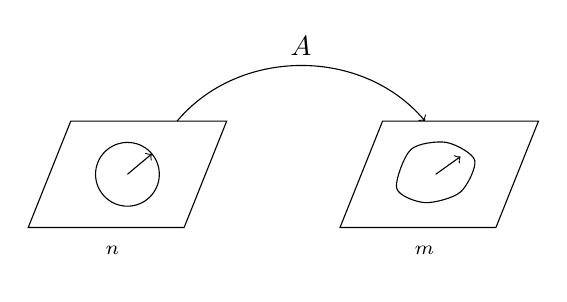
\begin{tikzpicture}[scale=0.9]
  % R^n parallelogram with unit ball
  \draw (0,0) -- (2.2,0) -- (2.8,1.5) -- (0.6,1.5) -- cycle;
  \draw (1.4,0.75) circle (0.45);
  \draw[->] (1.4,0.75) -- ++(40:0.45);
  \node at (1.2,-0.4) {$\R^n$};
  % R^m parallelogram with image of the unit ball
  \draw (4.4,0) -- (6.6,0) -- (7.2,1.5) -- (5.0,1.5) -- cycle;
  \draw plot[smooth cycle] coordinates {(5.2,0.55) (5.6,0.35) (6.1,0.5) (6.3,0.95) (5.9,1.2) (5.4,1.1)};
  \draw[->] (5.75,0.75) -- (6.1,1.0);
  \node at (5.6,-0.4) {$\R^m$};
  % mapping arrow
  \draw[->] (2.1,1.5) to[out=50,in=130] node[above] {$A$} (5.6,1.5);
\end{tikzpicture}
\end{center}

% ===== Page 14 =====
\origpage{14}
\begin{example}
Consider an $m\times n$ matrix with real elements. Choose $\ell_\infty$-norm $\norm{\cdot}_\infty$ for both $\R^n$ \& $\R^m$.
\[
\norm{A}_\infty = \max_{\norm{x}_\infty=1} \norm{Ax}_\infty,
\qquad
A = \bmat{1 & -2\\ -3 & 4\\ -2 & 2},
\qquad x\in\R^2,\quad y = Ax \in \R^3
\]
\[
\norm{x}_\infty = \max(|x_1|,|x_2|) = 1
\]
\begin{center}
\begin{minipage}{0.4\textwidth}
\centering
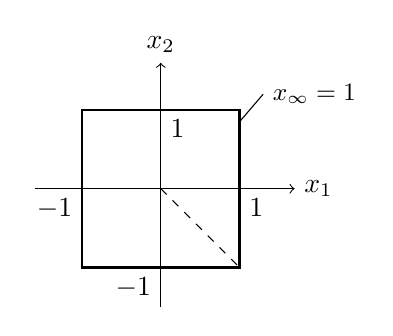
\begin{tikzpicture}[scale=1.0]
  \draw[->] (-1.6,0) -- (1.7,0) node[right] {$x_1$};
  \draw[->] (0,-1.5) -- (0,1.6) node[above] {$x_2$};
  \draw[thick] (-1,-1) rectangle (1,1);
  \node[below left] at (-1,0) {$-1$};
  \node[below right] at (1,0) {$1$};
  \node[below right] at (0,1) {$1$};
  \node[below left] at (0,-1) {$-1$};
  \draw[dashed] (0,0) -- (1,-1);
  \draw (1,0.85) -- (1.3,1.2) node[right,font=\small] {$\norm{x}_\infty=1$};
\end{tikzpicture}
\end{minipage}%
\begin{minipage}{0.55\textwidth}
First row only:
\[
A_1 = \bmat{1 & -2}\bmat{x_1\\ x_2}
\]
\[
\max_{\norm{x}_\infty=1} |A_1 x| = \max_{\norm{x}_\infty=1} |x_1 - 2x_2| = 3
\]
\explain{Attained at $x_1 = 1$, $x_2 = -1$ (dashed corner).}
\end{minipage}
\end{center}
For the whole matrix:
\begin{align*}
Ax &= \bmat{x_1 - 2x_2\\ -3x_1 + 4x_2\\ -2x_1 + 2x_2}\\
\norm{Ax}_\infty &= \max\big(|x_1 - 2x_2|,\ |-3x_1+4x_2|,\ |-2x_1+2x_2|\big)\\
x^* &= \bmat{1\\ -1} \quad\text{or}\quad x^* = \bmat{-1\\ 1}\\
Ax^* &= \bmat{3\\ -7\\ -4} \;\Rightarrow\; \norm{Ax^*}_\infty = 7
\end{align*}
\[
\underline{\underline{\norm{A}_\infty = 7}}
\]
\end{example}
\begin{keybox}
\[
\norm{A}_\infty = \max_i \sum_{j=1}^n |a_{ij}| \qquad \text{(max row sum)}
\]
\end{keybox}
\begin{insight}[Why the max row sum]
If $\norm{x}_\infty = 1$ then $|x_j|\le 1$ for all $j$, so for each row
$|(Ax)_i| = \big|\sum_j a_{ij}x_j\big| \le \sum_j |a_{ij}||x_j| \le \sum_j |a_{ij}|$.
Hence $\norm{Ax}_\infty\le\max_i\sum_j|a_{ij}|$. Equality is reached by taking the row $i^*$ with the largest sum and $x_j = \operatorname{sign}(a_{i^*j})$ (a corner of the square). In the example the row sums are $3,7,4$ and row 2 $= [-3\ \ 4]$ gives $x^* = [-1\ \ 1]\T$ (or its negative).
\end{insight}

\sep
\paragraph{$\ell_1$-norm.}
\[
\norm{A}_1 = \max_{\norm{x}_1=1}\norm{Ax}_1, \qquad \norm{x}_1 = |x_1| + |x_2| = 1
\]
\begin{center}
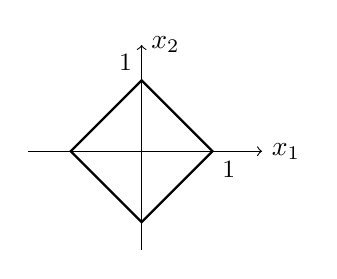
\begin{tikzpicture}[scale=0.9]
  \draw[->] (-1.6,0) -- (1.7,0) node[right] {$x_1$};
  \draw[->] (0,-1.4) -- (0,1.5) node[right] {$x_2$};
  \draw[thick] (1,0) -- (0,1) -- (-1,0) -- (0,-1) -- cycle;
  \node[below right,font=\small] at (1,0) {$1$};
  \node[above left,font=\small] at (0,1) {$1$};
\end{tikzpicture}
\end{center}
\begin{align*}
A_1 &= \bmat{1 & -2}\\
A_1 x &= x_1 - 2x_2\\
\norm{A_1 x} &= |x_1 - 2x_2|\\
\max_{\norm{x}_1 = 1}\norm{A_1 x} &= \max_{\norm{x}_1 = 1} |x_1 - 2x_2|
\end{align*}
\explain{Weighted average of $1$ and $-2$: on $\norm{x}_1=1$, $|x_1 - 2x_2| \le |x_1| + 2|x_2| \le 2(|x_1|+|x_2|) = 2$, so the best is to put all the weight on the entry of largest magnitude.}
\needspace{7\baselineskip}
\begin{align*}
x &= \bmat{0.5\\ -0.5} \quad\Rightarrow\quad \tfrac12 + 1 = \tfrac32\\
x &= \bmat{0.2\\ -0.8} \quad\Rightarrow\quad \text{larger}\\
x &= \bmat{0\\ -1} \quad\Rightarrow\quad \text{largest:}\quad \underline{\norm{A_1x} = 2}
\end{align*}

% ===== Page 15 =====
\origpage{15}
Now the whole matrix:
\[
A = \bmat{1 & -2\\ -3 & 4\\ -2 & 2}, \qquad
Ax = \bmat{1\\ -3\\ -2}x_1 + \bmat{-2\\ 4\\ 2}x_2
\]
\[
\norm{Ax}_1 = \Bigg\|\underbrace{\bmat{1\\ -3\\ -2}}_{6}x_1 + \underbrace{\bmat{-2\\ 4\\ 2}}_{8\ \checkmark}x_2\Bigg\|_1 = 8
\qquad (x_1 = 0,\ x_2 = 1)
\]
% corrected: notes have a stray "7" written below the "8"; the value of ||A||_1 is 8 (column sums 6 and 8); 7 is ||A||_inf from the previous page
\explain{Column sums: $|1|+|-3|+|-2| = 6$ and $|-2|+|4|+|2| = 8$, so $\norm{A}_1 = 8$ (compare $\norm{A}_\infty = 7$: different vector norms give different matrix norms).}
\begin{keybox}
\[
\norm{A}_1 = \max_j \sum_i |a_{ij}| \qquad \text{(max column sum)}
\]
\end{keybox}
\begin{insight}[Why the max column sum]
Write $A = [a_1\ \cdots\ a_n]$ by columns. If $\norm{x}_1 = 1$,
$\norm{Ax}_1 = \big\|\sum_j x_j a_j\big\|_1 \le \sum_j |x_j|\,\norm{a_j}_1 \le \big(\max_j\norm{a_j}_1\big)\sum_j|x_j| = \max_j\norm{a_j}_1$,
with equality for $x = e_{j^*}$ (a corner of the diamond), $j^*$ the column of largest absolute sum.
\end{insight}

\subsection{Convergence of Sequences}\label{ss:convergence}
\begin{definition}
Let $(\V,\F,\norm{\cdot})$ be a normed space. Let $\{v_n\}_{n=1}^\infty$ be a sequence of vectors in $\V$, i.e., $v_n\in\V\ \forall n$. The sequence $\{v_n\}_{n=1}^\infty$ is said to \term{converge} to the \term{limit} $\boxed{v\in\V}$ iff
\[
\boxed{\norm{v_n - v} \to 0 \quad \text{as } n\to\infty}
\]
\end{definition}
\begin{remark}
A sequence is \term{divergent} if it is not convergent.
\end{remark}
\begin{example}
$\V = \R$, $\norm{v} = |v|$.

\paragraph{Sequence $v_n = (1/2)^n$.} Candidate limit $v = 0 \in \V$:
\begin{align*}
\norm{v_n - v} &= \left|\frac{1}{2^n} - 0\right| = \frac{1}{2^n}\\
\lim_{n\to\infty}\norm{v_n - v} &= 0
\;\Rightarrow\; v_n \to 0 \text{ as } n\to\infty
\end{align*}

\paragraph{Sequence $v_n = (-1)^n$.} Try $v = 0$:
\[
\norm{(-1)^n - 0} = |(-1)^n| = 1, \qquad \lim_{n\to\infty}\overbrace{\norm{v_n - v}}^{1} = 1 \neq 0
\]
\explain{The sequence does not converge to $v = 0$.}
Try $v = 1$:
\[
\norm{(-1)^n - 1} = \abs{(-1)^n - 1} = \begin{cases} 0, & n \text{ even}\\ 2, & n \text{ odd}\end{cases} \;\Rightarrow\; \text{does not converge}
\]
% corrected: notes had ||(-1)^n - 1|| = (-1)^n - 1 (absolute value missing; that expression is negative for odd n)
\explain{The distance keeps jumping back to $2$, so it does not tend to $0$.}
$\therefore$ \key{Sequence is not convergent anywhere.}
\begin{insight}
For an arbitrary candidate $v\in\R$: the even terms are $1$ and the odd terms are $-1$, so by the triangle inequality $2 = |1-(-1)| \le |v_{2k}-v| + |v - v_{2k+1}|$. Thus at least one of two consecutive distances is $\ge 1$, and $\norm{v_n - v}\not\to 0$ for every $v$.
\end{insight}
\end{example}

\begin{example}
$\V = \left\{ f : [-1,1]\to\R \;\middle|\; f(\cdot) \text{ is continuous}, \ \int_{-1}^{1}|f(t)|\,dt < \infty \right\}$
\[
\norm{f(\cdot)} = \int_{-1}^{1} |f(t)|\,dt \qquad (\mathcal{L}_1 \text{ norm})
\]
% corrected: notes had the integral over (-infinity, infinity); functions in V live on [-1,1]
Is $f_n$ convergent?
\begin{align*}
f_n(t) &= e^{-n|t|}, \quad n\ge 0\\
f_0(t) &= e^{0t} = 1\\
f_1(t) &= e^{-|t|}\\
f_2(t) &= e^{-2|t|}\\
&\ \,\vdots
\end{align*}

% ===== Page 16 =====
\origpage{16}
\begin{center}
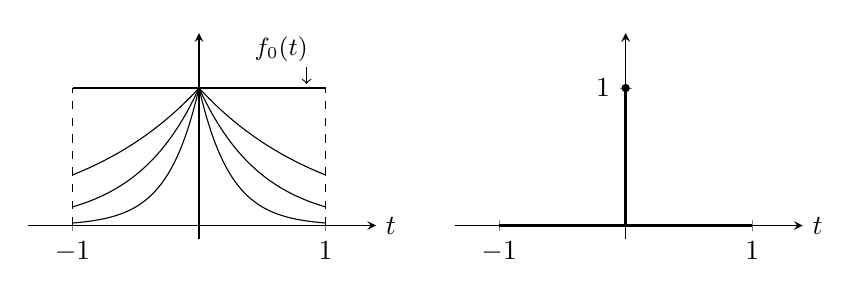
\begin{tikzpicture}
\begin{axis}[name=left,width=6cm,height=4.2cm,axis lines=middle,
  xmin=-1.35,xmax=1.4,ymin=-0.1,ymax=1.4,xtick={-1,1},ytick=\empty,
  xlabel={$t$},clip=false,every axis x label/.style={at={(current axis.right of origin)},anchor=west}]
  \addplot[thick,domain=-1:1] {1};
  \addplot[dashed] coordinates {(-1,0) (-1,1)};
  \addplot[dashed] coordinates {(1,0) (1,1)};
  \foreach \n in {1,2,4} {
    \addplot[domain=-1:1,samples=81] {exp(-\n*abs(x))};
  }
  \node[above,font=\small] at (axis cs:0.65,1.12) {$f_0(t)$};
  \draw[->] (axis cs:0.85,1.15) -- (axis cs:0.85,1.03);
\end{axis}
\begin{axis}[at={(left.east)},anchor=west,xshift=1cm,width=6cm,height=4.2cm,axis lines=middle,
  xmin=-1.35,xmax=1.4,ymin=-0.1,ymax=1.4,xtick={-1,1},ytick={1},
  xlabel={$t$},every axis x label/.style={at={(current axis.right of origin)},anchor=west}]
  \addplot[very thick] coordinates {(-1,0) (1,0)};
  \addplot[very thick] coordinates {(0,0) (0,1)};
  \addplot[only marks,mark=*,mark size=1.3pt] coordinates {(0,1)};
\end{axis}
\end{tikzpicture}
\end{center}
\explain{Left: $f_0, f_1, f_2, f_4$. Right: pointwise limit as $n\to\infty$ ($0$ for $t\neq0$, $1$ at $t=0$) $\notin \V$ (not continuous).}

\begin{center}
\begin{minipage}{0.32\textwidth}
\centering
\begin{tikzpicture}
\begin{axis}[width=4.6cm,height=3.2cm,axis lines=middle,
  xmin=-1.35,xmax=1.4,ymin=-0.3,ymax=1.2,xtick={-1,1},ytick=\empty]
  \addplot[very thick] coordinates {(-1,0) (1,0)};
\end{axis}
\end{tikzpicture}

$0(t)\in\V$
\end{minipage}%
\begin{minipage}{0.64\textwidth}
Candidate limit: the zero function $0(t)$.\\ $v\in\V$ is satisfied \checkmark
\end{minipage}
\end{center}
\begin{align*}
\norm{f_n(t) - 0(t)} &= \norm{f_n(t)} = \int_{-1}^{1}\left|e^{-n|t|}\right|dt\\
&= \int_{-1}^{1} e^{-n|t|}\,dt
&&\text{(exponential is positive)}\\
&= 2\cdot\int_0^1 e^{-nt}\,dt
&&\text{(even function)}\\
&= 2\,\frac{e^{-nt}}{-n}\bigg|_0^1 = -2\left(\frac{e^{-n}}{n} - \frac1n\right)\\
\norm{f_n(t) - 0(t)} &= -\frac{2}{n}\big(\underbrace{e^{-n} - 1}_{\to -1}\big) = \frac{2\,(1-e^{-n})}{n} \le \frac2n\\
\lim_{n\to\infty}\norm{f_n(t) - 0(t)} &= 0 \;\Rightarrow\; \norm{v_n - v}\to 0 \text{ as } n\to\infty \ \checkmark
\end{align*}
$\therefore$ \key{It is convergent to the zero function.}
\end{example}

\needspace{6\baselineskip}
\sep
\key{Convergence depends on the distance definition} (the norm):
\begin{itemize}[nosep]
\item for the $\mathcal{L}_1$ norm $\Rightarrow$ convergent
\item for the $\mathcal{L}_\infty$ (sup) norm $\Rightarrow$ divergent
\end{itemize}
\begin{insight}
With $\norm{f}_\infty = \max_{-1\le t\le 1}|f(t)|$ we get $\norm{f_n - 0}_\infty = \max_t e^{-n|t|} = 1$ (at $t=0$) for every $n$, so $f_n\not\to 0$. No other continuous $g$ works either: $\norm{f_n - g}_\infty\to0$ would force $g(t) = \lim_n f_n(t)$ pointwise, i.e.\ $g(0)=1$ and $g(t)=0$ for $t\neq0$, which is not continuous. The $\mathcal L_1$ norm only ``sees'' area, and the area under the narrowing peak vanishes; the $\mathcal L_\infty$ (sup) norm sees the peak height, which stays $1$.
\end{insight}

\subsection{Cauchy Sequences and Completeness}\label{ss:cauchy}
\begin{definition}
Let $(\V,\F,\norm{\cdot})$ be a normed space. A sequence $\{v_n\}_{n=0}^\infty$ is said to be a \term{Cauchy sequence} iff
\[
\lim_{n,m\to\infty}\norm{v_n - v_m} = 0
\]
\end{definition}
\begin{claim}
\key{Every convergent sequence is a Cauchy sequence.} The reverse statement, in general, is not correct.
\[
\text{Convergent} \;\underset{\not\Leftarrow}{\Rightarrow}\; \text{Cauchy}
\]
\end{claim}
\begin{proof}
Suppose that $\{v_n\}_{n=0}^\infty$ is convergent to $v\in\V$, i.e.\ $\lim_{n\to\infty}\norm{v_n - v} = 0$. Then
\begin{align*}
\lim_{n,m\to\infty}\norm{v_n - v_m} &= \lim_{n,m\to\infty}\norm{v_n - v + v - v_m}\\
&\le \lim_{n,m\to\infty} \big(\norm{v_n - v} + \norm{v - v_m}\big)\\
&= \underbrace{\lim_{n\to\infty}\norm{v_n - v}}_{=0} + \underbrace{\lim_{m\to\infty}\norm{v_m - v}}_{=0} = 0
\end{align*}
\explain{Inequality step: triangle inequality, $\norm{a+b}\le\norm{a}+\norm{b}$ with $a = v_n - v$, $b = v - v_m$.}
\[
0 \le \lim_{n,m\to\infty}\norm{v_n - v_m} \le 0 \;\Rightarrow\; \lim_{n,m\to\infty}\norm{v_n - v_m} = 0 \;\Rightarrow\; \{v_n\} \text{ is Cauchy.}
\qedhere
\]
\end{proof}
% corrected: notes justified the inequality step "by absolute convergence"; it is the triangle inequality (and ||v - v_m|| = ||v_m - v|| by homogeneity with alpha = -1)

% ===== Page 17 =====
\origpage{17}
\begin{example}
$\V = \Q$: set of rational numbers, $\F = \Q$ as well.
\[
\sqrt{2} = 1.41421356237310\ldots \;\Rightarrow\; \text{not a rational number}
\]
\begin{align*}
v_0 &= 1 = \tfrac11\\
v_1 &= 1.4 = \tfrac{14}{10}\\
v_2 &= 1.41 = \tfrac{141}{100}\\
v_3 &= 1.414 = \tfrac{1414}{1000}\\
&\ \,\vdots
\end{align*}
We need $v\in\V$ s.t.\ $\norm{v_n - v}\to 0$ as $n\to\infty$, where $v_n \in\V\ \forall n$.
But $v$ should be $\sqrt2$ for $\norm{v_n - v}\to 0$ as $n\to\infty$.
\begin{center}
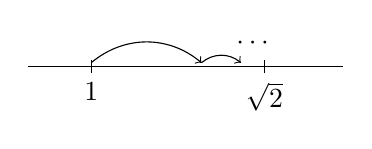
\begin{tikzpicture}
  \draw (0,0) -- (4,0);
  \draw (0.8,0.08) -- (0.8,-0.08) node[below] {$1$};
  \draw (3,0.08) -- (3,-0.08) node[below] {$\sqrt2$};
  \draw[->] (0.8,0.05) to[out=40,in=140] (2.2,0.05);
  \draw[->] (2.2,0.05) to[out=40,in=140] (2.7,0.05);
  \node at (2.85,0.3) {$\cdots$};
\end{tikzpicture}
\end{center}
Since $\sqrt2\notin\V$, $\therefore\ \{v_n\}$ is not convergent (in $\V$).

\paragraph{What about Cauchyness?}
\[
\norm{v_n - v_m} \to 0 \text{ as } n,m\to\infty
\]
$v_n$ is actually Cauchy as elements are approaching each other.
\explain{Indeed $v_n$ and $v_m$ agree in the first $\min(n,m)$ decimals, so $|v_n - v_m| < 10^{-\min(n,m)} \to 0$.}
\[
\therefore\ \text{\key{Convergent $\Rightarrow$ Cauchy}} \quad\text{but}\quad \text{Cauchy} \not\Rightarrow \text{Convergent}
\]
\explain{Margin note (Turkish): ``ben bi sequence olsam sana converge ederdim.''}
\end{example}
If a set does not have holes $\Rightarrow$ \key{complete} set.
\begin{insight}
The same sequence viewed in $\V=\R$ converges (to $\sqrt2\in\R$): convergence depends on the space, not only on the terms. $\R$ is complete (it ``fills the holes'' of $\Q$), and so is every finite-dimensional normed space over $\R$ or $\C$, e.g.\ $(\R^n,\norm{\cdot}_p)$. Incompleteness is therefore a phenomenon of infinite-dimensional spaces such as function spaces, as the next example shows.
\end{insight}

\begin{definition}
A normed space is said to be \term{complete} iff \key{every Cauchy sequence is convergent}. A complete normed space is called a \term{Banach space}.
\end{definition}
\begin{example}
A normed space defined as
\[
\V = \left\{ f(\cdot) \;\middle|\; f:[-1,1]\to\R,\ f \text{ is continuous } \& \int_{-1}^{1}|f(t)|\,dt < \infty\right\},
\qquad
\norm{f}_1 = \int_{-1}^{1}|f(t)|\,dt
\]
Consider the sequence $\{f_n\}_{n=1}^\infty$:
\[
f_n(t) = \begin{cases} 1, & -1\le t\le 0\\ 1 - nt, & 0\le t\le \frac1n\\ 0, & \frac1n\le t\le 1\end{cases}
\]
\begin{center}
\pgfplotsset{fnplot/.style={width=4.6cm,height=3.4cm,axis lines=middle,
  xmin=-1.3,xmax=1.35,ymin=-0.15,ymax=1.35,ytick={1},
  yticklabel style={anchor=south west,font=\small},
  every axis y label/.style={at={(current axis.above origin)},anchor=south west}}}
\begin{tikzpicture}
\begin{axis}[fnplot,name=a1,xtick={-1,1},ylabel={$f_1(t)$},xlabel={$t$},
  every axis x label/.style={at={(current axis.right of origin)},anchor=west}]
  \addplot[thick] coordinates {(-1,0) (-1,1) (0,1) (1,0)};
\end{axis}
\begin{axis}[fnplot,name=a2,at={(a1.east)},anchor=west,xshift=0.6cm,
  xtick={-1,0.5,1},xticklabels={$-1$,$\frac12$,$1$},ylabel={$f_2(t)$}]
  \addplot[thick] coordinates {(-1,0) (-1,1) (0,1) (0.5,0) (1,0)};
\end{axis}
\node at ($(a2.east)+(0.35,0)$) {$\cdots$};
\begin{axis}[fnplot,name=a3,at={(a2.east)},anchor=west,xshift=0.7cm,
  xtick={-1,0.25,1},xticklabels={$-1$,$\frac1n$,$1$},ylabel={$f_n(t)$}]
  \addplot[thick] coordinates {(-1,0) (-1,1) (0,1) (0.25,0) (1,0)};
\end{axis}
\end{tikzpicture}
\end{center}
Is the sequence $\{f_n\}$ Cauchy? Convergent?
\[
\norm{f_n(t) - f_m(t)}_1 = \int_{-1}^{1}|f_n(t) - f_m(t)|\,dt
\]
\begin{center}
\begin{minipage}{0.45\textwidth}
\centering
\begin{tikzpicture}
\begin{axis}[width=5.4cm,height=3.8cm,axis lines=middle,
  xmin=-1.3,xmax=1.35,ymin=-0.15,ymax=1.3,ytick={1},yticklabel style={anchor=south west},
  xtick={-1,0.3,0.6,1},xticklabels={$-1$,$\frac1m$,$\frac1n$,$1$},clip=false]
  \addplot[pattern=north east lines,draw=none] coordinates {(0,1) (0.6,0) (0.3,0) (0,1)};
  \addplot[thick] coordinates {(-1,0) (-1,1) (0,1) (0.6,0) (1,0)};
  \addplot[thick] coordinates {(0,1) (0.3,0)};
  \draw (axis cs:0.33,0.45) -- (axis cs:0.75,0.95) node[right,font=\small,align=left] {difference\\integration\\is this area.};
\end{axis}
\end{tikzpicture}
\end{minipage}%
\begin{minipage}{0.5\textwidth}
\[
\text{Area} = \left|\frac1n - \frac1m\right|\cdot\frac12
\]
\explain{Triangle with vertices $(0,1)$, $(\frac1m,0)$, $(\frac1n,0)$: base $|\frac1n-\frac1m|$, height $1$.}
\[
\lim_{n,m\to\infty}\left|\frac1n - \frac1m\right|\cdot\frac12 = 0
\]
\end{minipage}
\end{center}
\begin{center}
\begin{minipage}{0.45\textwidth}
\centering
\begin{tikzpicture}
\begin{axis}[width=5.4cm,height=3.8cm,axis lines=middle,
  xmin=-1.3,xmax=1.35,ymin=-0.15,ymax=1.3,ytick={1},yticklabel style={anchor=south west},
  xtick={-1,0,1},title={$f_n \xrightarrow{\,n\to\infty\,}$},title style={font=\small}]
  \addplot[thick] coordinates {(-1,0) (-1,1) (0,1) (0,0) (1,0)};
\end{axis}
\end{tikzpicture}
\end{minipage}%
\begin{minipage}{0.5\textwidth}
The limit $\notin\V$ (not continuous).

$\Rightarrow \{f_n\}$ is Cauchy but not convergent.

$\therefore$ \key{$(\V,\F,\norm{\cdot}_1)$ is not complete.}
\end{minipage}
\end{center}
\begin{insight}
To be precise, ``not convergent'' means no \emph{continuous} $g$ satisfies $\norm{f_n - g}_1\to 0$. If one did, then on $[-1,0]$ we would need $\int_{-1}^0|1-g|\,dt = 0$, so $g = 1$ there; and on every $[\delta,1]$, $\delta>0$, $f_n = 0$ eventually, so $g = 0$ there. Then $g$ jumps at $t = 0$, contradicting continuity. The ``limit'' is the step function, which lies outside $\V$.
\end{insight}
\end{example}

% ===== Page 18 =====
\origpage{18}
\paragraph{Now with $(\V,\F,\norm{\cdot}_\infty)$.}
\begin{align*}
\norm{f}_\infty &= \max_{-1\le t\le 1}|f(t)|\\
\norm{f_n(t) - f_m(t)}_\infty &= \max_{-1\le t\le 1}|f_n(t) - f_m(t)|
\end{align*}
\begin{center}
\begin{minipage}{0.4\textwidth}
\begin{align*}
f_n(t) &= 1 - nt \quad \big(0\le t\le\tfrac1n\big)\\
f_n\!\left(\tfrac1m\right) &= 1 - \frac nm \quad (m\ge n)
\end{align*}
\end{minipage}%
\begin{minipage}{0.5\textwidth}
\centering
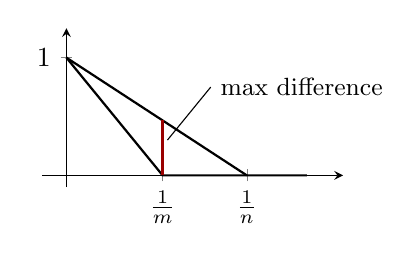
\begin{tikzpicture}
\begin{axis}[width=5.4cm,height=3.6cm,axis lines=middle,
  xmin=-0.1,xmax=1.15,ymin=-0.1,ymax=1.25,ytick={1},
  xtick={0.4,0.75},xticklabels={$\frac1m$,$\frac1n$},clip=false]
  \addplot[thick] coordinates {(0,1) (0.4,0) (1,0)};
  \addplot[thick] coordinates {(0,1) (0.75,0)};
  \addplot[very thick,red!60!black] coordinates {(0.4,0) (0.4,{1-0.4/0.75})};
  \draw (axis cs:0.42,0.3) -- (axis cs:0.6,0.75) node[right,font=\small] {max difference};
\end{axis}
\end{tikzpicture}
\end{minipage}
\end{center}
% corrected: notes wrote lim_{n,m} ||f_n - f_m||_inf = |1 - n/m|; the distance itself equals |1 - n/m| (m >= n), and this does not tend to 0
\begin{align*}
\norm{f_n(t) - f_m(t)}_\infty &= f_n\!\left(\tfrac1m\right) - \underbrace{f_m\!\left(\tfrac1m\right)}_{0} = {\underbrace{\left|1 - \frac nm\right|}_{\neq 0 \text{ unless } n=m}} \qquad (m\ge n)\\
\text{e.g.\ } m = 2n:\quad \norm{f_n - f_{2n}}_\infty &= \tfrac12 \quad \text{for every } n
\end{align*}
\begin{center}
\fbox{\begin{minipage}{0.75\textwidth}\small\itshape
$n$ ve $m$'in nasıl $\infty$'a gittiği fark etmez, her zaman limit sonucu sıfır olmalı. Bu senaryoda if $n=m$ o zaman limit sıfır, onun dışında değil.
\end{minipage}}
\end{center}
% translation: it does not matter how n and m go to infinity, the limit must always be zero.
% In this scenario the limit is zero only if n = m, not otherwise.
\explain{It does not matter how $n$ and $m$ go to $\infty$; the limit must always be zero. Here it is zero only if $n=m$.}
\explain{The maximum is at $t=\frac1m$: on $[0,\frac1m]$ the difference $(m-n)t$ increases, and on $[\frac1m,\frac1n]$ it equals $1-nt$, which decreases.}
$\therefore$ \key{$\{f_n\}$ is not Cauchy} in the sup norm.

\needspace{16\baselineskip}
\section{Inner Product Spaces}\label{sec:ips}
\syllabusweek{Week 4 --- inner product spaces, orthogonality, Gram--Schmidt}
\subsection{Inner Products}\label{ss:inner-products}
\begin{definition}
Let $(\V,\C)$ be a vector space. An \term{inner product} is a function from $\V\times\V$ into $\C$,
\[
\inner{\cdot}{\cdot} : \V\times\V\to\C
\]
satisfying the following properties:
\begin{enumerate}[label=\arabic*)]
\item $\inner{x}{y} = \overline{\inner{y}{x}}$ \quad $\forall x,y\in\V$ \hfill (conjugate symmetry)
\item Linearity with respect to (wrt) the first argument:
  \begin{enumerate}[label=\alph*)]
  \item $\inner{x+y}{z} = \inner{x}{z} + \inner{y}{z}$ \quad $\forall x,y,z\in\V$ \hfill (additivity)
  \item $\inner{\alpha x}{y} = \alpha\inner{x}{y}$ \quad $\forall\alpha\in\C$ and $\forall x,y\in\V$ \hfill (homogeneity)
  \end{enumerate}
\item $\inner{x}{x}$ is real \& nonnegative, $\inner{x}{x}\ge 0$, and
  $\inner{x}{x} = 0 \Leftrightarrow x = 0_{\V}$ \hfill (positive definiteness)
\end{enumerate}
$\therefore$ The triplet $(\V,\C,\inner{\cdot}{\cdot})$ is called an \term{inner product space}.
\end{definition}
\begin{align*}
\inner{x}{y+z} &= \overline{\inner{y+z}{x}} = \overline{\inner{y}{x}} + \overline{\inner{z}{x}} = \inner{x}{y} + \inner{x}{z}
\end{align*}
\explain{Additivity wrt second argument \checkmark}
\begin{align*}
\inner{x}{\alpha y} &= \overline{\inner{\alpha y}{x}} = \bar\alpha\,\overline{\inner{y}{x}} = \bar\alpha\inner{x}{y}
\end{align*}
\explain{Homogeneity wrt second argument $\times$ ($\alpha$ should be real). We have \key{conjugate homogeneity wrt second argument}.}
\begin{insight}
So an inner product is linear in the first argument and \emph{conjugate}-linear in the second:
$\inner{\textstyle\sum_i\alpha_i x_i}{\sum_j\beta_j y_j} = \sum_{i,j}\alpha_i\bar\beta_j\inner{x_i}{y_j}$.
Over $\F=\R$ the conjugates disappear and the inner product is bilinear and symmetric. Also $\inner{x}{0_\V} = \inner{0_\V}{x} = 0$ for all $x$ (take $\alpha = 0$ in homogeneity).
\end{insight}

% ===== Page 19 =====
\origpage{19}
\begin{example}
$\V = \C^n$, $\F = \C$, \quad
$x = [x_1\ x_2 \ldots x_n]\T$, \ $y = [y_1\ y_2 \ldots y_n]\T$, \quad $x_i, y_i\in\C$.
\[
\inner{x}{y} = \sum_{i=1}^n x_i\bar y_i = \bar y\T x = y\Hm x
\qquad \Big(\begin{bmatrix} \bar y_1 & \bar y_2 & \cdots\end{bmatrix}\bmat{x_1\\ x_2\\ \vdots}\Big)
% corrected: notes had the row vector [y_1 y_2 ...]; y^H = conj(y)^T has conjugated entries
\]
Check the axioms:
\begin{enumerate}[label=\arabic*)]
\item $\inner{x}{y} = \sum_{i=1}^n x_i\bar y_i = \bar y\T x = y\Hm x$
\[
\overline{\inner{y}{x}} = \overline{x\Hm y} = \overline{\bar x\T y} = \underbrace{x\T\bar y = \bar y\T x}_{\text{scalar} = \text{its transpose}} = y\Hm x = \inner{x}{y}
\]
\item \begin{enumerate}[label=\alph*)]
  \item $\inner{x+y}{z} = z\Hm(x+y) = z\Hm x + z\Hm y = \inner{x}{z} + \inner{y}{z}$
  \item $\inner{\alpha x}{y} = y\Hm(\alpha x) = \alpha y\Hm x = \alpha\inner{x}{y}$
  \end{enumerate}
\item $\inner{x}{x} = x\Hm x = \sum_{i=1}^n |x_i|^2 \ge 0 \;\Rightarrow$ real value;
  \ $\inner{x}{x} = 0 \Leftrightarrow x = 0_\V$.
\end{enumerate}
\end{example}
\begin{example}
$A, B\in\R^{m\times n}$, \ $\V=\R^{m\times n}$, \ $\F=\R$, \ $A = [a_{ij}]$, \ $B = [b_{ij}]$:
\[
\inner{A}{B} = \sum_{i,j} a_{ij}b_{ij}
\]
\[
\underbrace{\bmat{a_{11} & a_{12} & a_{13}\\ a_{21} & a_{22} & a_{23}}\cdot
\bmat{b_{11} & b_{21}\\ b_{12} & b_{22}\\ b_{13} & b_{23}}}_{A\cdot B\T}
=
\bmat{a_{11}b_{11} + a_{12}b_{12} + a_{13}b_{13} & \times\\ \times & a_{21}b_{21} + a_{22}b_{22} + a_{23}b_{23}}
\]
% corrected: notes had B^T with rows b11 b12 / b12 b22 / b13 b23 (entry (1,2) must be b21)
\begin{align*}
\inner{A}{B} &\triangleq \tr(AB\T)\\
&= \tr(A\T B) \quad \text{(in the real field)}
\end{align*}
\explain{$(AB\T)_{ii} = \sum_j a_{ij}b_{ij}$ (row $i$ of $A$ against row $i$ of $B$), so the trace adds up all $a_{ij}b_{ij}$; the off-diagonal entries ($\times$) are irrelevant. For complex matrices one uses $\inner{A}{B} = \tr(AB\Hm) = \tr(B\Hm A)$, whose induced norm is the Frobenius norm.}
\end{example}
\begin{example}
$\V = \left\{ f(\cdot) \;\middle|\; f:[0,1]\to\C \text{ s.t. } \int_0^1 |f(t)|^2\,dt < \infty\right\}$
\[
\inner{f_1}{f_2} \triangleq \int_0^1 f_1(t)\overline{f_2(t)}\,dt \qquad (\mathcal{L}_2 \text{ inner product})
\]
\end{example}
\subsection{The Cauchy--Schwarz Inequality and the Induced Norm}\label{ss:cauchy-schwarz}
\begin{theorem}[Cauchy--Schwarz Inequality]
Let $\V$ be an inner product space. Let $x,y\in\V$.
\[
|\inner{x}{y}|^2 \le \inner{x}{x}\inner{y}{y}
\]
Equality holds iff $x = cy$ for some $c\in\C$ or $y = 0_\V$, i.e.\ \key{equality iff $x$ and $y$ are linearly dependent}.
\end{theorem}
% corrected: notes stated equality iff x = cy; the case y = 0_V (x arbitrary) also gives equality 0 = 0, so the condition is linear dependence
\paragraph{Equality check for $x = cy$.}
\begin{align*}
\inner{x}{y} &= \inner{cy}{y} = c\inner{y}{y} \;\Rightarrow\; |\inner{x}{y}|^2 = |c|^2\inner{y}{y}^2\\
\inner{x}{x} &= \inner{cy}{cy} = c\bar c\inner{y}{y} = |c|^2\inner{y}{y} \qquad (c\bar c = |c|^2 \text{ is real})
\end{align*}
\explain{Using the first- and second-argument axioms.}
\[
\underbrace{|c|^2\inner{y}{y}^2}_{|\inner{x}{y}|^2} = \underbrace{|c|^2\inner{y}{y}}_{\inner{x}{x}}\underbrace{\inner{y}{y}}_{\inner{y}{y}}
\]

% ===== Page 20 =====
\origpage{20}
\begin{proof}[Proof of theorem]
\textbf{Case 1: $y = 0_{\V}$.}
\begin{align*}
\inner{x}{y} &= \inner{x}{0_{\V}} = \inner{x}{0\cdot 0_{\V}} = 0\cdot\inner{x}{0_{\V}} = 0\\
\inner{y}{y} &= 0 \quad \text{(by axioms)}\\
\underbrace{|\inner{x}{y}|^2}_{0} &\le \underbrace{\inner{x}{x}}_{\ge 0}\underbrace{\inner{y}{y}}_{0} \;\Rightarrow\; 0\le 0 \ \checkmark
\end{align*}

\textbf{Case 2: $y\neq 0_{\V}$.} Then $\inner{y}{y}\neq 0$ (in fact $\inner{y}{y}>0$ by axiom 3, so we may divide by it and multiply inequalities by it).
For $\alpha\in\C$ (in field):
\begin{align*}
0 &\le \inner{x-\alpha y}{x-\alpha y}\\
&= \inner{x}{x} - \inner{x}{\alpha y} - \inner{\alpha y}{x} + \inner{\alpha y}{\alpha y}\\
&= \inner{x}{x} - \bar\alpha\inner{x}{y} - \alpha{\underbrace{\inner{y}{x}}_{\overline{\inner{x}{y}}}} + |\alpha|^2\inner{y}{y}
\end{align*}
Choose $\displaystyle \alpha = \frac{\inner{x}{y}}{\inner{y}{y}}$:
\begin{align*}
0 &\le \inner{x}{x} - \frac{\overline{\inner{x}{y}}}{\inner{y}{y}}\cdot\inner{x}{y} - \cancel{\frac{\inner{x}{y}}{\inner{y}{y}}\cdot\overline{\inner{x}{y}}} + \cancel{\frac{|\inner{x}{y}|^2}{\inner{y}{y}^2}\cdot\inner{y}{y}}\\
0 &\le \inner{x}{x} - \frac{|\inner{x}{y}|^2}{\inner{y}{y}}\\
\frac{|\inner{x}{y}|^2}{\inner{y}{y}} &\le \inner{x}{x} \;\Rightarrow\; \therefore\ |\inner{x}{y}|^2 \le \inner{x}{x}\inner{y}{y}
\qedhere
\end{align*}
\end{proof}
\begin{insight}[Choice of $\alpha$ and the equality case]
$\alpha y$ with $\alpha = \inner{x}{y}/\inner{y}{y}$ is the projection of $x$ onto $y$ (see Gram--Schmidt below), so $x-\alpha y\perp y$ and the first line says $\norm{x-\alpha y}^2\ge 0$: the error of the best approximation of $x$ along $y$ has nonnegative length.
Equality in the theorem (with $y\neq 0_\V$) holds iff $\inner{x-\alpha y}{x-\alpha y} = 0$, i.e.\ iff $x = \alpha y$ by axiom 3. This proves the ``only if'' part of the equality statement; the ``if'' part is the check for $x = cy$ above.
\end{insight}

\begin{remark}
An inner product \key{induces a norm} (the \term{induced norm}) defined as
\[
\norm{x}^2 \triangleq \inner{x}{x}, \qquad \norm{x} \triangleq \sqrt{\inner{x}{x}}
\]
\end{remark}
\paragraph{Show that this is a norm.}
\begin{enumerate}[label=\arabic*)]
\item $\norm{x}\ge 0$, \ $\norm{x} = 0 \Leftrightarrow x = 0_{\V}$ \checkmark \ (by axiom 3 of the inner product) \hfill (positive definiteness)
\item $\displaystyle \norm{\alpha x} \triangleq \sqrt{\inner{\alpha x}{\alpha x}} = \sqrt{\alpha\cdot\bar\alpha\inner{x}{x}}
= |\alpha|\underbrace{\sqrt{\inner{x}{x}}}_{\norm{x}} = |\alpha|\norm{x}$ \checkmark \hfill (absolute homogeneity)
\item $\norm{x+y} = \sqrt{\inner{x+y}{x+y}}$ \hfill (triangle inequality)
\begin{align*}
\norm{x+y}^2 &= \inner{x+y}{x+y} = \inner{x}{x} + \inner{x}{y} + {\underbrace{\inner{y}{x}}_{\overline{\inner{x}{y}}}} + \inner{y}{y}\\
&= \inner{x}{x} + 2\cdot\operatorname{Re}\inner{x}{y} + \inner{y}{y}\\
&\le \inner{x}{x} + 2|\operatorname{Re}\inner{x}{y}| + \inner{y}{y}\\
&\le \inner{x}{x} + 2|\inner{x}{y}| + \inner{y}{y}
\intertext{\origpage{21}By Cauchy--Schwarz, $|\inner{x}{y}| \le \sqrt{\inner{x}{x}\inner{y}{y}}$:}
% ===== Page 21 =====
&\le \inner{x}{x} + 2\sqrt{\inner{x}{x}}\sqrt{\inner{y}{y}} + \inner{y}{y}\\
&= \left(\sqrt{\inner{x}{x}} + \sqrt{\inner{y}{y}}\right)^2\\
&= (\norm{x} + \norm{y})^2\\
\norm{x+y}^2 &\le (\norm{x} + \norm{y})^2 \;\Rightarrow\; \norm{x+y}\le\norm{x}+\norm{y} \ \checkmark
\end{align*}
\explain{Both sides are nonnegative, so taking square roots preserves the inequality: the triangle inequality holds.}
\end{enumerate}

\sep
\paragraph{Angle between vectors.} By Cauchy--Schwarz, $|\inner{x}{y}| \le \norm{x}\norm{y}$; \ suppose $x\neq 0_{\V}$, $y\neq 0_{\V}$:
\[
0 \le \frac{|\inner{x}{y}|}{\norm{x}\norm{y}} \le 1
\]
\[
\cos\theta \triangleq \frac{|\inner{x}{y}|}{\norm{x}\norm{y}} \;\Rightarrow\; \theta = \arccos\left(\frac{|\inner{x}{y}|}{\norm{x}\norm{y}}\right)
\]
\explain{Cauchy--Schwarz is exactly what makes this angle well defined. With the absolute value $\theta\in[0,\frac\pi2]$; in a real space one often drops it, $\cos\theta = \frac{\inner{x}{y}}{\norm{x}\norm{y}}\in[-1,1]$, which for $\R^2,\R^3$ is the usual geometric angle. $\theta = \frac\pi2$ $\Leftrightarrow$ $\inner{x}{y}=0$ (orthogonal), $\theta = 0$ $\Leftrightarrow$ $x = cy$.}
\begin{remark}
\key{Every inner product space is also a normed space.} The converse/reverse is not correct in general.
\end{remark}
\begin{insight}
A norm comes from an inner product \key{iff it satisfies the parallelogram law}
$\norm{x+y}^2 + \norm{x-y}^2 = 2\norm{x}^2 + 2\norm{y}^2$.
For example $\norm{\cdot}_1$ on $\R^2$ fails it: $x = e_1$, $y = e_2$ give $4+4 = 8 \neq 4 = 2+2$. So $\ell_1$ and $\ell_\infty$ are norms without an inner product behind them; only $\ell_2$ is induced by $\inner{x}{y} = y\T x$.
\end{insight}
\begin{definition}
An inner product space that is complete wrt the induced norm is called a \term{complete inner product space} / \term{Hilbert space}.
\end{definition}
\subsection{Orthogonality and Orthogonal Expansions}\label{ss:orthogonality}
\begin{definition}
Two vectors $x,y\in\V$ are said to be \term{orthogonal} iff $\inner{x}{y} = 0$.
Similarly subsets $S_1, S_2\subset\V$ are orthogonal iff $\inner{x}{y} = 0$ $\forall x\in S_1$, $\forall y\in S_2$.
\end{definition}
\paragraph{Examples.}
\begin{enumerate}[label=\arabic*)]
\item $\V=\R^n$, $\F=\R$, \quad $\inner{x}{y} = \sum_{i=1}^n x_iy_i = y\T x = x\T y$
\[
\underbrace{B = \{e_1, e_2, \ldots, e_n\}}_{\text{canonical basis set}} \qquad
e_1 = \bmat{1\\ 0\\ \vdots\\ 0} \quad e_2 = \bmat{0\\ 1\\ 0\\ \vdots\\ 0} \quad \cdots
\]
\[
\inner{e_i}{e_j} = \begin{cases} 0, & i\neq j\\ 1, & i = j\end{cases} = \delta_{ij}
\]
\item $\V = \left\{ f(\cdot) \;\middle|\; f:[-\pi,\pi]\to\C \text{ s.t. } \int_{-\pi}^{\pi}|f(t)|^2\,dt < \infty\right\}$

Consider $\{e^{jnt}\}_{n=-\infty}^{\infty}$, \quad $e^{jnt}\in\V$ for all $n$.
\[
\inner{f_1(t)}{f_2(t)} = \int_{-\pi}^{\pi} f_1(t)\,\overline{f_2(t)}\,dt
\]
\begin{align*}
\inner{e^{jnt}}{e^{jmt}} &= \int_{-\pi}^{\pi} e^{jnt}\,e^{-jmt}\,dt = \int_{-\pi}^{\pi} e^{j(n-m)t}\,dt\\
&= \int_{-\pi}^{\pi}\big[\cos((n-m)t) + j\sin((n-m)t)\big]\,dt\\
% ===== Page 22 =====
&= \int_{-\pi}^{\pi}\cos((n-m)t)\,dt + j\underbrace{\cancel{\int_{-\pi}^{\pi}\sin((n-m)t)\,dt}}_{0}
\end{align*}
\origpage{22}
\begin{center}
\begin{minipage}{0.5\textwidth}
\small $\left.\begin{array}{l}\sin t\\ \sin 2t\\ \sin 3t\\ \ \vdots\end{array}\right\}$ all zero due to integral over a period
\end{minipage}%
\begin{minipage}{0.35\textwidth}
\centering
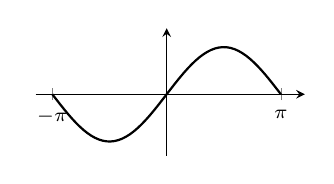
\begin{tikzpicture}
\begin{axis}[width=5cm,height=3.2cm,axis lines=middle,
  xmin=-3.6,xmax=3.8,ymin=-1.3,ymax=1.4,xtick={-3.1416,3.1416},xticklabels={$-\pi$,$\pi$},
  ytick=\empty,tick label style={font=\scriptsize}]
  \addplot[thick,domain=-pi:pi,samples=60] {sin(deg(x))};
\end{axis}
\end{tikzpicture}
\end{minipage}
\end{center}
\begin{align*}
\inner{e^{jnt}}{e^{jmt}} &= \begin{cases} 2\pi, & n = m\\ 0, & n\neq m\end{cases}\\
&= 2\pi\,\delta_{nm}
\end{align*}
\explain{For $n=m$: $\int_{-\pi}^{\pi}\cos 0\,dt = 2\pi$. For $k = n-m\neq0$: $\int_{-\pi}^{\pi}\cos kt\,dt = \frac{2\sin k\pi}{k} = 0$, and $\int_{-\pi}^{\pi}\sin kt\,dt = 0$ since $\sin kt$ is odd.}
\item $S_1 = \{\sin nt\}_{n=1}^\infty$, \ $S_2 = \{\cos mt\}_{m=1}^\infty$:
\begin{align*}
\inner{\sin nt}{\cos mt} &= \int_{-\pi}^{\pi}\sin nt\cdot\cos mt\,dt\\
&= \int_{-\pi}^{\pi}\frac12\Big(\underbrace{\cancel{\sin((n+m)t)}}_{0} + \underbrace{\cancel{\sin((n-m)t)}}_{0}\Big)\,dt = 0
\end{align*}
\explain{Product-to-sum: $\sin a\cos b = \frac12[\sin(a+b)+\sin(a-b)]$; both terms are odd functions (or zero when $n=m$), so they integrate to $0$ over the symmetric interval $[-\pi,\pi]$.}
\[
\therefore\ \key{$S_1\perp S_2$}
\]
\end{enumerate}

\sep
\paragraph{Expansion in an orthogonal set.}
\begin{itemize}
\item[$\blacktriangleright$]
$z = \alpha_1 z_1 + \alpha_2 z_2$ \quad if $z_1\perp z_2$:
\begin{align*}
\inner{z}{z_1} &= \inner{\alpha_1 z_1 + \alpha_2 z_2}{z_1}\\
&= \alpha_1\inner{z_1}{z_1} + \alpha_2\underbrace{\cancel{\inner{z_2}{z_1}}}_{0} \;\Rightarrow\; \alpha_1 = \frac{\inner{z}{z_1}}{\inner{z_1}{z_1}}
\end{align*}
In general,
\[
z = \sum_{i=1}^n \alpha_i z_i, \qquad \alpha_i = \frac{\inner{z}{z_i}}{\inner{z_i}{z_i}} \quad \forall i
\]
\explain{Valid when $z\in\Span\{z_1,\ldots,z_n\}$ and the $z_i\neq 0_\V$ are mutually orthogonal: take $\inner{\cdot}{z_k}$ of both sides and all terms with $i\neq k$ vanish. \key{No linear system has to be solved; each coefficient is computed independently.}}
Example (as $z_1\perp z_2$):
\[
{\underbrace{\bmat{2\\ 3}}_{z}} = \beta_1{\underbrace{\bmat{1\\ 1}}_{z_1}} + \beta_2{\underbrace{\bmat{1\\ -1}}_{z_2}},
\qquad
\beta_1 = \frac{\inner{z}{z_1}}{\inner{z_1}{z_1}} = \frac{5}{2},
\qquad
\beta_2 = \frac{\inner{z}{z_2}}{\inner{z_2}{z_2}} = \frac{2-3}{2} = -\frac12
\]
\explain{Check: $\frac52\bmat{1\\1} - \frac12\bmat{1\\-1} = \bmat{2\\3}$ \checkmark}
\item[$\blacktriangleright$]
$f(t) = \sum_{n=-\infty}^{\infty}\alpha_n e^{jnt}$:
\[
\alpha_n = \frac{\inner{f(t)}{e^{jnt}}}{\inner{e^{jnt}}{e^{jnt}}} = \frac{1}{2\pi}\int_{-\pi}^{\pi} f(t)e^{-jnt}\,dt \qquad \text{(Fourier series coefficients)}
\]
\explain{With $\inner{f_1}{f_2} = \int_{-\pi}^{\pi} f_1(t)\,\overline{f_2(t)}\,dt$.}
\end{itemize}

% ===== Page 23 =====
\subsection{Gram--Schmidt Orthogonalization}\label{ss:gram-schmidt}
\origpage{23}%
\paragraph{Question.} Let $\V$ be an inner product space. Let $S_1 = \{v_1, v_2, \ldots, v_n\}$ be a linearly independent set. Can we obtain another set $S_2 = \{w_1, w_2, \ldots, w_n\}$ s.t.
\begin{enumerate}[label=\arabic*)]
\item $w_i\perp w_j$ when $i\neq j$
\item $\Span\{S_1\} = \Span\{S_2\}$?
\end{enumerate}
\key{Yes!} (constructively, by the following algorithm)

\needspace{16\baselineskip}
\paragraph{Gram--Schmidt orthogonalization algorithm.} The $w_k$ are constructed one at a time.
\paragraph{Step 1.} $w_1 = v_1$

\paragraph{Step 2.} $\displaystyle w_2 = v_2 - \frac{\inner{v_2}{w_1}}{\inner{w_1}{w_1}}\cdot w_1$
\begin{align*}
\inner{w_2}{w_1} &= \inner{v_2 - \frac{\inner{v_2}{w_1}}{\inner{w_1}{w_1}}\cdot w_1}{w_1}\\
&= \cancel{\inner{v_2}{w_1}} - \underbrace{\frac{\cancel{\inner{v_2}{w_1}}}{\cancel{\inner{w_1}{w_1}}}}_{\text{scalar}}\cancel{\inner{w_1}{w_1}} = 0
\end{align*}
\begin{center}
\begin{minipage}{0.55\textwidth}
\centering
\begin{tikzpicture}[scale=1.5]
  \coordinate (O) at (0,0);
  \coordinate (V1) at (1,2.4);
  \coordinate (V2) at (2.6,0.7);
  % projection of v2 onto v1: k = <v2,v1>/<v1,v1>
  \pgfmathsetmacro{\k}{(1*2.6+2.4*0.7)/(1*1+2.4*2.4)}
  \coordinate (P) at ({\k*1},{\k*2.4});
  \draw[->,thick,blue!60!black] (O) -- (V1) node[above] {$v_1 = w_1$};
  \draw[->,thick] (O) -- (V2) node[right] {$v_2$};
  \draw[->,very thick,red!60!black] (O) -- (P);
  \draw[->,very thick,red!80!black] (O) -- ($(O)!0.42!(P)$);
  \node[red!60!black,left,font=\small] at ($(O)!0.25!(P)+(-0.05,0)$) {$\frac{w_1}{\norm{w_1}}$};
  \draw[->,thick] (P) -- (V2) node[midway,above right] {$w_2$};
  \draw[dashed,red!60!black] (P) -- (V2);
  % right-angle mark at P
  \draw ($(P)!0.12cm!(V2)$) -- ($(P)!0.12cm!(V2)+(P)!0.12cm!(V1)-(P)$) -- ($(P)!0.12cm!(V1)$);
  \node[red!60!black,left,font=\small] at ($(P)+(-0.45,0.25)$) {$\frac{\inner{v_2}{w_1}}{\inner{w_1}{w_1}}\cdot w_1$};
  \draw[->,red!60!black] ($(P)+(-0.5,0.2)$) -- ($(P)+(-0.05,0.02)$);
  \pic[draw,"$\theta$",angle radius=0.45cm,angle eccentricity=1.45] {angle = V2--O--V1};
\end{tikzpicture}
\end{minipage}%
\begin{minipage}{0.4\textwidth}
\[
\inner{x}{y} = \norm{x}\norm{y}\cos\theta
\]
\end{minipage}
\end{center}
\[
\frac{\inner{v_2}{w_1}}{\underbrace{\inner{w_1}{w_1}}_{\norm{w_1}^2}}\cdot w_1
= \frac{\inner{v_2}{w_1}}{\norm{w_1}}\cdot\frac{w_1}{\norm{w_1}}
= \underbrace{\inner{v_2}{\frac{w_1}{\norm{w_1}}}}_{\norm{v_2}\cos\theta}\frac{w_1}{\norm{w_1}}
\]

\paragraph{Step 3.} $\displaystyle w_3 = v_3 - \frac{\inner{v_3}{w_1}}{\inner{w_1}{w_1}}\cdot w_1 - \frac{\inner{v_3}{w_2}}{\inner{w_2}{w_2}}\cdot w_2$
\[
\frac{\inner{v_i}{w_j}}{\inner{w_j}{w_j}}\cdot w_j \;:\; \text{\term{projection} of } v_i \text{ onto } w_j
\]

\paragraph{Step $n$.} $\displaystyle w_n = v_n - \sum_{i=1}^{n-1}\frac{\inner{v_n}{w_i}}{\inner{w_i}{w_i}}\cdot w_i$
\begin{insight}[Why Gram--Schmidt works]
\emph{Orthogonality} (by induction): if $w_1,\ldots,w_{k-1}$ are mutually orthogonal, then for $j<k$
$\inner{w_k}{w_j} = \inner{v_k}{w_j} - \sum_{i<k}\frac{\inner{v_k}{w_i}}{\inner{w_i}{w_i}}\inner{w_i}{w_j} = \inner{v_k}{w_j} - \inner{v_k}{w_j} = 0$,
since only the $i=j$ term survives.
\emph{Same span}: each $w_k$ is $v_k$ minus a combination of $w_1,\ldots,w_{k-1}\in\Span\{v_1,\ldots,v_{k-1}\}$, so $\Span\{w_1,\ldots,w_k\} = \Span\{v_1,\ldots,v_k\}$ for every $k$.
\emph{No division by zero}: $w_k = 0_\V$ would make $v_k\in\Span\{v_1,\ldots,v_{k-1}\}$, impossible for a linearly independent $S_1$; so $\inner{w_k}{w_k}>0$.
In words: \key{$w_k$ is the component of $v_k$ orthogonal to the span of the previous vectors.}
\end{insight}

\begin{example}
$\V = \left\{ f \;\middle|\; f:[-1,1]\to\R,\ \int_{-1}^{1}(f(t))^2\,dt < \infty\right\}$, \quad $\F = \R$,
\[
\inner{f}{g} = \int_{-1}^{1} f(t)g(t)\,dt
\]
\[
S_1 = \{v_1, v_2, v_3\}, \qquad v_1(t) = 1, \quad v_2(t) = t, \quad v_3(t) = t^2,
\qquad\text{i.e.}\quad S_1 = \{1, t, t^2\}
\]

% ===== Page 24 =====
\origpage{24}
\begin{align*}
w_1 &= v_1 = 1\\
w_2 &= t - \frac{\overset{0}{\cancel{\inner{t}{1}}}}{\inner{1}{1}}\cdot 1 = t, \qquad \inner{t}{1} = \int_{-1}^{1} t\,dt = 0\\
w_3 &= t^2 - \frac{\inner{t^2}{1}}{\inner{1}{1}}\cdot 1 - \frac{\overset{0}{\cancel{\inner{t^2}{t}}}}{\inner{t}{t}}\cdot t = t^2 - \frac{2/3}{2} = t^2 - \frac13
\end{align*}
using
\begin{align*}
\inner{t^2}{1} &= \int_{-1}^{1} t^2\,dt = 2\int_0^1 t^2\,dt = \frac23\\
\inner{1}{1} &= \int_{-1}^{1} 1\,dt = 2\\
\inner{t^2}{t} &= \int_{-1}^{1} t^3\,dt = 0\\
\inner{t}{t} &= \int_{-1}^{1} t^2\,dt = \frac23
\end{align*}
\begin{center}
\begin{minipage}{0.45\textwidth}
\[
S_2 = \left\{1,\ t,\ t^2 - \tfrac13\right\}
\]
\centering \term{Legendre polynomials}
\end{minipage}%
\begin{minipage}{0.5\textwidth}
\centering
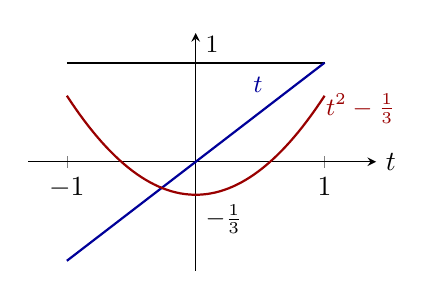
\begin{tikzpicture}
\begin{axis}[width=6cm,height=4.6cm,axis lines=middle,
  xmin=-1.3,xmax=1.4,ymin=-1.1,ymax=1.3,xtick={-1,1},ytick=\empty,xlabel={$t$},
  every axis x label/.style={at={(current axis.right of origin)},anchor=west},clip=false]
  \addplot[thick,domain=-1:1] {1};
  \node[above right,font=\small] at (axis cs:0,1) {$1$};
  \node[below right,font=\small] at (axis cs:0,-0.3333) {$-\frac13$};
  \addplot[thick,domain=-1:1,blue!60!black] {x} node[pos=0.8,above left,font=\small] {$t$};
  \addplot[thick,domain=-1:1,samples=60,red!60!black] {x^2-1/3} node[pos=0.95,right,font=\small] {$t^2-\frac13$};
\end{axis}
\end{tikzpicture}
\end{minipage}
\end{center}
\explain{Check: $\inner{t^2-\frac13}{1} = \frac23 - \frac13\cdot 2 = 0$ and $\inner{t^2-\frac13}{t} = \int_{-1}^1 (t^3 - \frac t3)\,dt = 0$ (odd integrand) \checkmark. These are the Legendre polynomials up to scaling: the standard ones are $P_0 = 1$, $P_1 = t$, $P_2 = \frac12(3t^2-1) = \frac32\big(t^2-\frac13\big)$, normalised so that $P_k(1) = 1$.}
\end{example}

\needspace{9\baselineskip}
\sep
\paragraph{Linearly dependent vectors.} If the vectors are linearly dependent, e.g.\ $S_1 = \{v_1, v_1\}$:
\begin{align*}
w_1 &= v_1\\
w_2 &= v_1 - \frac{\overset{1}{\cancel{\inner{v_1}{v_1}}}}{\cancel{\inner{v_1}{v_1}}}\cdot v_1 = 0
\end{align*}
\explain{When this is the case, \key{remove the redundant vector and resume the process}. In general $w_k = 0_\V$ exactly when $v_k$ depends linearly on $v_1,\ldots,v_{k-1}$; discarding such vectors, Gram--Schmidt returns an orthogonal basis of $\Span\{S_1\}$ (and its size is $\dim\Span\{S_1\}$).}

\needspace{12\baselineskip}
\paragraph{Gram--Schmidt orthonormalization.}
Require $\norm{w_i} = 1$, i.e.\ $\inner{w_i}{w_i} = 1$:
\begin{alignat*}{2}
\bar w_1 &= v_1, &\qquad w_1 &= \frac{\bar w_1}{\norm{\bar w_1}}\\*
\bar w_2 &= v_2 - \inner{v_2}{w_1}w_1, &\qquad w_2 &= \frac{\bar w_2}{\norm{\bar w_2}}\\*
&\ \,\vdots\\*
\bar w_n &= v_n - \sum_{i=1}^{n-1}\inner{v_n}{w_i}w_i, &\qquad w_n &= \frac{\bar w_n}{\norm{\bar w_n}}
\end{alignat*}
% corrected: notes had w_2 = \bar w_2 / ||w_2||; the normalisation divides by ||\bar w_2||. The last normalisation w_n = \bar w_n/||\bar w_n|| is implied by the pattern and added.
\explain{Since $\inner{w_i}{w_i} = 1$, the projection coefficients $\frac{\inner{v_k}{w_i}}{\inner{w_i}{w_i}}$ simplify to $\inner{v_k}{w_i}$. The resulting set is \term{orthonormal}: $\inner{w_i}{w_j} = \delta_{ij}$.}

\needspace{16\baselineskip}
\section{Linear Transformations}\label{sec:lt}
\syllabusweek{Week 5 --- linear transformations, null space, range space, matrix representations}
\subsection{Definition and Examples}\label{ss:lt-def}
\begin{definition}
Let $\V$ \& $\W$ be two vector spaces over the same field $\F$. A \term{linear transformation} $\mathcal{A}$ is a mapping from $\V$ into $\W$ shown as $\mathcal{A}:\V\to\W$ s.t.
\[
\mathcal{A}(\alpha_1 v_1 + \alpha_2 v_2) = \alpha_1\mathcal{A}v_1 + \alpha_2\mathcal{A}v_2
\]
for all $v_1,v_2\in\V$ and all $\alpha_1,\alpha_2\in\F$.
\end{definition}
\begin{center}
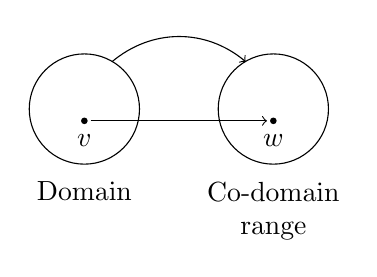
\begin{tikzpicture}
  \draw (0,0) circle (0.7);
  \draw (2.4,0) circle (0.7);
  \node at (0,0.35) {$\V$};
  \node at (2.4,0.35) {$\W$};
  \fill (0,-0.15) circle (1.2pt); \node at (0,-0.4) {$v$};
  \fill (2.4,-0.15) circle (1.2pt); \node at (2.4,-0.4) {$w$};
  \draw[->] (0.08,-0.15) -- (2.32,-0.15);
  \draw[->] (0.35,0.6) to[out=40,in=140] (2.05,0.6);
  \node[below] at (0,-0.8) {Domain};
  \node[below,align=center] at (2.4,-0.8) {Co-domain\\ range};
\end{tikzpicture}
\end{center}
\explain{$\V$ is the \term{domain} and $\W$ the \term{co-domain}; the \term{range} $\Range(\mathcal A) = \{\mathcal A v : v\in\V\}$ is the subset of $\W$ actually reached (in general $\Range(\mathcal A)\subseteq\W$).}
\begin{insight}
The single condition is equivalent to additivity $\mathcal A(v_1+v_2) = \mathcal Av_1+\mathcal Av_2$ together with homogeneity $\mathcal A(\alpha v) = \alpha\mathcal Av$. Taking $\alpha_1=\alpha_2=0$ gives $\mathcal A 0_\V = 0_\W$. Standard examples: $x\mapsto Ax$ for $A\in\F^{m\times n}$ ($\V=\F^n$, $\W=\F^m$, as in the induced-norm section), differentiation $f\mapsto f'$ on polynomials, and $f\mapsto\int_0^1 f(t)\,dt$.
\end{insight}
